\documentclass[10pt,a4paper,twocolumn]{article}
\usepackage[a4paper,margin=2.0cm,columnsep=0.6cm]{geometry}
\usepackage[T1]{fontenc}
\usepackage{mathptmx}
\usepackage{microtype}
\usepackage{amsmath,amssymb}
\usepackage{graphicx}
\usepackage{booktabs}
\usepackage{array}
\usepackage{multirow}
\usepackage{xcolor}
\usepackage{enumitem}
\usepackage{tikz}
\usetikzlibrary{positioning,arrows.meta,fit,backgrounds}
\usepackage[numbers,sort&compress]{natbib}
\usepackage[colorlinks=true,linkcolor=blue!50!black,citecolor=blue!50!black,urlcolor=blue!50!black]{hyperref}
\setlist{nosep,leftmargin=*}
\setlength{\textfloatsep}{8pt plus 2pt minus 2pt}
\setlength{\floatsep}{6pt plus 2pt minus 2pt}
\setlength{\abovecaptionskip}{3pt}
\newcommand{\1}{\mathbb{1}}
\newcommand{\B}{\mathcal{B}}
\newcommand{\C}{\mathcal{C}}

\title{\vspace{-1.2em}\textbf{Learned Controllers for Latent-Preserving Context Switching\\in Multi-Agent LM Dialogue}\\[2pt]
\large Mid-Evaluation Report --- Team \texttt{5MinsBoss}}
\author{Jai Aakash Gopalakrishnan \quad Aditya Nair \quad Chiranjeevi K \quad Rashmiraj Patra\\
IIIT Hyderabad}
\date{\vspace{-1.5em}}

\begin{document}
\maketitle

\begin{abstract}
When a third person joins a conversation, people often change the surface topic while still conveying their real meaning to each other. We study a controlled LM version of this behaviour. A speaker $A$ and an insider $B$ share a hidden topic $z$. When an outsider $C$ joins, $A$ must switch topic so that $B$ can still recover $z$ while $C$ cannot. A small \emph{discrete controller} chooses the cover topic for a frozen 1.5B-parameter LM. It is trained with REINFORCE on the reward $R=\1[B\text{ recovers }z]-\lambda\,\1[C\text{ recovers }z]$.
For the mid-evaluation we built a fully audited prototype. It includes a synthetic dataset with family-level splits, three non-learned baselines, a supervised insider decoder, a prompted outsider, four information controls, and one REINFORCE run at $\lambda=1$.
On 80 held-out test scenarios (160 rollouts per method) the RL controller reaches a mean reward of $0.494$ [95\% CI $0.41$, $0.58$]. The comparison methods score $0.225$ (prompt-only switching), $0.269$ (untrained controller) and $0.338$ (scripted switching). Joint success (B right, C wrong) is $0.50$, against at most $0.41$ for the baselines.
Our controls show that this gain is real but narrow. The controller converges to a near-deterministic, history-conditional choice of cover topic. That choice helps the \emph{trained} reward decoder (which goes from $0.45$ on history alone to $0.64$) but not a prompted insider. A decoder trained only on the public transcript still recovers $z$ at $0.30$, more than twice chance, so the hiding is far from secure. All results are preliminary (single seed, single $\lambda$, small test set).
\end{abstract}

%=====================================================================
\section{Introduction}
Humans routinely tailor what they say to who is listening. \citet{clark1987concealing} showed that speakers can conceal meaning from an overhearer while keeping it clear to an addressee, by relying on common ground the overhearer lacks. Sociolinguists describe the same phenomenon in terms of \emph{footing} and \emph{ratified} versus \emph{unratified} hearers \citep{goffman1981forms}, and in-group code-switching \citep{gumperz1982discourse}. A familiar example is two friends who stop discussing a surprise party when the guest of honour walks in, and start ``talking about gardening'' in a way that still lands for both of them.

Multi-agent LM systems now routinely place several agents in one conversation \citep{park2023generative,li2023camel,du2024debate}. This raises a parallel question for language models: can a small learned module teach frozen LMs to switch topic when an outsider arrives, without losing the latent information the insiders share? The question connects three lines of work. The first is zero-shot coordination (ZSC), where agents must coordinate through conventions under a shared latent signal \citep{hu2020otherplay,cui2021klevel}. The second is emergent communication between learned agents \citep{lazaridou2017multiagent,baroni2022tutorial}. The third is covert channels and steganography in generated text \citep{ziegler2019neural,wu2024generative,motwani2024secret}. Our reward has the same structure as the Alice--Bob--Eve objective of adversarial neural cryptography \citep{abadi2016learning}. The difference is that the ``cipher'' must operate through a frozen LM's \emph{discourse-level topic choice}, not learned bit encodings.

\paragraph{Mid-evaluation contributions.}
\begin{enumerate}
\item A \textbf{formal, refined problem statement} with explicit information boundaries for $A$, $B$, $C$ and the controller (\S\ref{sec:problem}).
\item A \textbf{literature review} positioning the project and arguing for its viability (\S\ref{sec:lit}).
\item A \textbf{reproducible prototype}, consisting of:
  \begin{itemize}
  \item an 8-topic benign synthetic dataset with leakage-safe splits;
  \item no-switch, scripted and prompt-only baselines;
  \item a frozen supervised $B$ decoder and a prompted $C$;
  \item a discrete REINFORCE controller;
  \item four information controls, 11 unit tests and three automated audits (\S\ref{sec:method}).
  \end{itemize}
\item \textbf{Initial results} with uncertainty estimates, controls and error analysis, reported honestly, including a negative result for the prompted insider (\S\ref{sec:results}).
\item A \textbf{revised timeline} for the rest of the project (\S\ref{sec:timeline}).
\end{enumerate}

%=====================================================================
\section{Problem Statement}\label{sec:problem}
\paragraph{Entities.} Let $\mathcal{Z}=\{1,\dots,K\}$ be a fixed set of hidden topics ($K{=}8$). Let $\mathcal{A}$ be a shared inventory of cover topics ($|\mathcal{A}|{=}8$). A scenario consists of a hidden topic $z\in\mathcal{Z}$ and a pre-switch history $h$ (four turns between $A$ and $B$). At the switch point, outsider $C$ joins. Then:
\begin{align*}
a &\sim \pi_\theta(\cdot \mid z, \phi(h)) && \text{(controller)}\\
m &\sim p_{\text{LM}}(\cdot \mid h, z, \iota(a)) && \text{(A's message)}\\
\hat z_B &= \B(h, m),\ \ \hat z_C = \C(m) && \text{(decoders)}
\end{align*}
Here $\phi$ is a \emph{frozen} LM feature map of the history. $\iota(a)$ is an explicit natural-language instruction (``Switch the conversation to \emph{board games} \ldots''). $p_{\text{LM}}$ is a frozen instruction-tuned LM. The controller maximises
\begin{equation}
J(\theta)=\mathbb{E}_{z,h,a,m}\big[\1[\hat z_B{=}z]-\lambda\,\1[\hat z_C{=}z]\big],
\label{eq:obj}
\end{equation}
so $R\in\{-1,0,1\}$ for $\lambda=1$. Only $\theta$ is trained, never the base LM.

\paragraph{Theoretical grounding in Rational Speech Acts (RSA).}
We formally ground our objective in the Rational Speech Acts (RSA) framework \citep{frank2012predicting,goodman2016pragmatic}. In standard RSA, a pragmatic speaker $S_1$ chooses an utterance $u$ to maximise communicative utility for a listener, balancing informativeness against production cost: $U(u; z) = \log L(z \mid u) - c(u)$. When generalized to multi-party settings featuring an unratified overhearer or eavesdropper $C$ alongside the intended, ratified recipient $B$ \citep{clark1987concealing,cohngordon2018pragmatically,hawkins2020continual}, the overhearer-aware pragmatic speaker optimizes:
\begin{equation}
U_{\text{RSA}}(u; z, h) = \log L_B(z \mid u, h) - \lambda \log L_C(z \mid u) - c(u).
\label{eq:rsa_obj}
\end{equation}
Here $L_B$ models the \emph{informed} insider whose posterior updates over $(h, u)$, whereas $L_C$ models the unratified outsider who observes only the public utterance $u$ (lacking the common ground history $h$). The cost term $c(u) \propto -\log p_{\text{LM}}(u \mid h)$ penalizes unnatural or unfluent utterances, enforcing \emph{linguistic naturalness}.

Direct Bayesian computation of $U_{\text{RSA}}$ requires marginalizing over the intractable space of all possible multi-turn continuations. In our framework, we instantiate this objective through reinforcement learning over a frozen foundation LM $p_{\text{LM}}$:
\begin{enumerate}
\item \textbf{0--1 communication reward as surrogate:} In decision-theoretic communication games with discrete topic recovery under $0$--$1$ loss, maximizing accuracy corresponds to minimizing Bayes risk. The empirical reward $R = \1[\hat z_B = z] - \lambda \1[\hat z_C = z]$ directly operationalises the tension between $B$'s informativeness and $C$'s obfuscation in Eq.~\eqref{eq:rsa_obj}.
\item \textbf{Informed $B$ vs.\ outsider $C$:} Agent $B$ is explicitly modeled as an informed listener by granting its decoder access to $(h, m)$, so that $h$ serves as shared private common ground \citep{clark1987concealing}. In contrast, outsider $C$ is restricted to public text $m$.
\item \textbf{Linguistic naturalness via frozen generation:} By restricting the controller to discrete natural-language cover instructions $\iota(a)$ and using a frozen foundation model $p_{\text{LM}}$ for surface generation, $c(m)$ is implicitly minimized, preserving fluency and preventing cryptographic language drift.
\end{enumerate}

\paragraph{Information boundaries.} These are enforced in code and checked by automated audits:
\begin{itemize}
\item $A$ and the controller know $z$. $A$ receives a private description of $z$ in its own prompt.
\item $B$ sees only $(h,\,[\text{C joins}],\,m)$.
\item $C$ sees only $([\text{C joins}],\,m)$, because it joins after the switch.
\item Neither $B$ nor $C$ ever receives $z$, its description, $a$, the controller state, or $A$'s prompt.
\item Both choose from the same complete, fixed-order list of $K$ labels.
\item Invalid answers are logged and scored as incorrect.
\end{itemize}
Figure~\ref{fig:flow} summarises the information flow. The primary measurement is taken immediately after $A$'s first post-switch message. We do not generate a $B$ reply, so $B$'s own reply cannot manufacture the signal being measured.

\begin{figure}[t]
\centering
\resizebox{\columnwidth}{!}{%
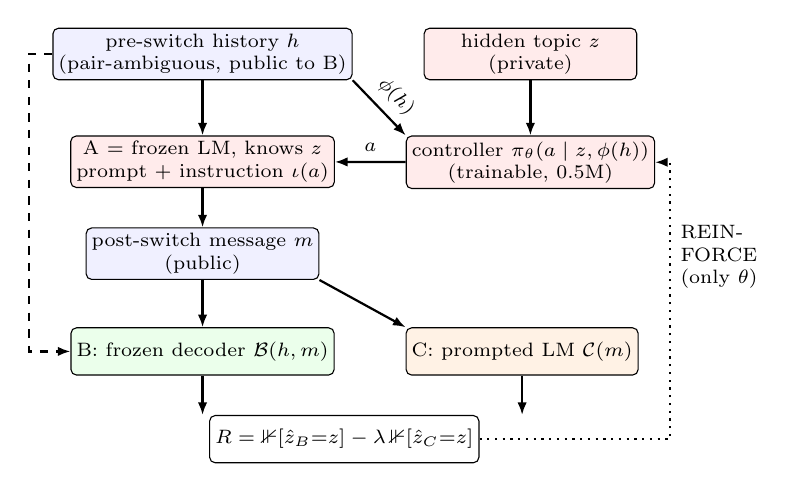
\begin{tikzpicture}[font=\scriptsize, node distance=5mm and 9mm,
  box/.style={draw, rounded corners=2pt, align=center, minimum height=6mm, minimum width=27mm, inner sep=2pt},
  priv/.style={box, fill=red!8}, pub/.style={box, fill=blue!6}, arr/.style={-{Latex[length=1.6mm]}, thick}]
\node[pub] (h) {pre-switch history $h$\\(pair-ambiguous, public to B)};
\node[priv, right=of h] (z) {hidden topic $z$\\(private)};
\node[priv, below=7mm of h] (A) {A = frozen LM, knows $z$\\prompt $+$ instruction $\iota(a)$};
\node[priv, below=7mm of z] (pi) {controller $\pi_\theta(a\mid z,\phi(h))$\\(trainable, 0.5M)};
\node[pub, below=of A] (m) {post-switch message $m$\\(public)};
\node[box, fill=green!8, below=6mm of m] (B) {B: frozen decoder $\mathcal{B}(h,m)$};
\node[box, fill=orange!10, right=of B] (C) {C: prompted LM $\mathcal{C}(m)$};
\node[box, below=5mm of B, xshift=18mm] (R) {$R=\mathbb{1}[\hat z_B{=}z]-\lambda\,\mathbb{1}[\hat z_C{=}z]$};
\draw[arr] (h) -- (A);
\draw[arr] (z) -- (pi);
\draw[arr] (h.south east) -- node[above, sloped, pos=.55]{$\phi(h)$} (pi.north west);
\draw[arr] (pi) -- node[above]{$a$} (A);
\draw[arr] (A) -- (m);
\draw[arr] (m) -- (B);
\draw[arr] (m.south east) -- (C.north west);
\draw[arr, dashed] (h.west) -- ++(-3mm,0) |- (B.west);
\draw[arr] (B.south) -- (R.north -| B.south);
\draw[arr] (C.south) -- (R.north -| C.south);
\draw[arr, dotted] (R.east) -| ([xshift=4mm]C.east) |- node[pos=.25, right, align=left]{REIN-\\FORCE\\(only $\theta$)} (pi.east);
\end{tikzpicture}}
\caption{Information flow. Red: private to A and the controller. Blue: public text. B additionally sees the history $h$ (dashed); C sees only $m$. Only the controller is trained.}
\label{fig:flow}
\end{figure}

\paragraph{Refinements relative to the proposal.}
\begin{enumerate}
\item \textbf{Pair-ambiguous histories.} Topics come in four pairs, for example \emph{surprise party} vs.\ \emph{farewell video}. Both topics of a pair share an \emph{identical} history string, so history alone can identify at most the pair (ceiling $0.5$, chance $0.125$). Any recovery above $0.5$ must come through $m$. This makes ``$B$ just remembers the earlier conversation'' measurable.
\item \textbf{Discrete conditioning.} The proposal left open whether to use a discrete cover choice or a soft prompt \citep{lester2021power}. We chose the discrete option for the mid-evaluation, because it is interpretable and auditable.
\item \textbf{Frozen $B$ decoder.} The proposal co-trained $B$'s head. We instead \emph{pre-train and freeze} it before RL, so the controller faces a stationary reward.
\item \textbf{Matched-information audit.} A decoder with $B$'s architecture and training access, but only $C$'s view, measures how much of the $B$--$C$ gap is decoder training rather than privileged context.
\end{enumerate}

\paragraph{Research questions (refined).}
\begin{itemize}
\item \textbf{RQ1:} Does a learned controller raise $B$'s recovery above scripted and prompt-only switching, beyond what history alone gives?
\item \textbf{RQ2:} Does it lower $C$'s recovery at matched conditions?
\item \textbf{RQ3:} How do these trade off as $\lambda$ varies? (post-mid)
\item \textbf{RQ4:} Is $z$ linearly decodable from controller representations when $C$ is at chance? (post-mid)
\end{itemize}

%=====================================================================
\section{Literature Review}\label{sec:lit}
\paragraph{Concealment, RSA, and audience design in human dialogue.}
\citet{clark1987concealing} studied speakers who must refer to objects so that a partner understands but an overhearer does not. They found that speakers exploit private common ground, and that overhearers do considerably worse than addressees. This is the human analogue of our $B$/$C$ asymmetry, and it motivates our use of pre-switch history as the insiders' shared key. Collaborative reference \citep{clark1986referring}, Goffman's participation framework \citep{goffman1981forms}, and conversational code-switching as an in-group signal \citep{gumperz1982discourse} supply the conceptual vocabulary. In computational pragmatics, the \emph{Rational Speech Acts} (RSA) framework \citep{frank2012predicting,goodman2016pragmatic} models communication as recursive probabilistic inference between speakers and listeners. Crucially, extensions of RSA to reference games with overhearers and unshared context \citep{cohngordon2018pragmatically,hawkins2020continual} show that speakers naturally calibrate informativeness against overhearer leakage. Our pair-ambiguous history design operationalises this exact dynamic.

\paragraph{Zero-shot coordination.}
In cooperative multi-agent RL, agents trained together often converge on arbitrary conventions that fail with new partners. \emph{Other-Play} \citep{hu2020otherplay} and K-level reasoning \citep{cui2021klevel} address this in Hanabi \citep{bard2020hanabi}, a game whose core difficulty is conveying hidden information through constrained, publicly observed actions. Human-AI coordination work \citep{carroll2019utility,strouse2021fcp} shows that self-play conventions can be brittle with real partners. Our results reproduce a small version of this phenomenon. The controller learns a convention that its own reward decoder understands but a prompted insider does not (\S\ref{sec:results}). This makes ZSC-style robustness a central concern for the second half of the project.

\paragraph{Emergent communication.}
Early work showed that agents can learn communication protocols from task reward \citep{foerster2016learning,lazaridou2017multiagent,havrylov2017emergence}. However, such protocols are rarely natural or compositional \citep{kottur2017natural,chaabouni2020compositionality}. Surveys \citep{lazaridou2020emergent,baroni2022tutorial} emphasise that grounding emergent protocols in natural language is an open problem. Fine-tuning a pretrained LM for communication causes \emph{language drift} \citep{lee2019countering,lu2020seeded}. Our design avoids drift by construction, because the LM is frozen and the controller acts only through natural-language instructions. Recent work on emergent coordination among LLM agents \citep{riedl2025emergent} suggests that such coordination can arise without weight updates, which supports a frozen-LM approach.

\paragraph{Adversarial cryptography and adversarial privacy.}
\citet{abadi2016learning} trained Alice and Bob to communicate while an adversary Eve tries to decode. Our reward is the dialogue analogue, with two key differences: the channel is natural language, and Eve ($C$) is a fixed, non-co-trained LM. In NLP, adversarial training has been used to remove protected attributes from representations \citep{ganin2016domain,elazar2018adversarial,coavoux2018privacy}. A recurring finding is that a \emph{post-hoc trained} probe recovers much of what the adversary appeared to remove \citep{elazar2018adversarial}. This finding directly motivated our public-transcript-trained decoder audit.

\paragraph{Linguistic steganography and LLM collusion.}
Text steganography hides bits in generated text, either through LSTM or LM sampling choices \citep{fang2017generating,ziegler2019neural,dai2019towards}, or with provable security under realistic distributions \citep{kaptchuk2021meteor}. \citet{wu2024generative} use LLMs for generative steganography. Watermarking \citep{kirchenbauer2023watermark} is the cooperative counterpart. These methods require token-level control and a shared secret key, whereas we operate through discourse-level topic choice. More recently, LLM agents have been shown to develop or be prompted into covert collusion \citep{motwani2024secret,mathew2024hidden}, and to encode hidden reasoning \citep{roger2023preventing}. These works frame covert channels as a safety risk. Our benign, small-scale setting offers a controlled testbed for measuring such channels, including how easily a \emph{trained} outsider detects them.

\paragraph{Steering frozen language models and representation engineering.}
A frozen LM can be steered in several ways: with control codes \citep{keskar2019ctrl}, attribute-model gradients \citep{dathathri2020pplm}, discriminator-guided decoding \citep{krause2021gedi}, continuous prefixes or soft prompts \citep{li2021prefix,lester2021power}, activation additions \citep{turner2023activation}, or RL-optimised discrete prompts \citep{deng2022rlprompt}. Concurrently, \emph{Representation Engineering} (RepE) \citep{zou2023representation}, \emph{Inference-Time Intervention} (ITI) \citep{li2023inference}, and latent steering vectors \citep{subramani2022extracting} show that internal activation spaces of frozen models can be directly controlled along conceptual directions without parameter updates. Our discrete controller sits at the intersection: it conditions on latent representations $\phi(h)$ and $z$ to select natural-language steering instructions with policy gradients.

\paragraph{RL with language-model environments.}
REINFORCE \citep{williams1992simple} and its sequence-level variants \citep{ranzato2016sequence} remain competitive for LM optimisation \citep{ahmadian2024back}, alongside PPO-based RLHF \citep{schulman2017ppo,ouyang2022training}. Because our action space is small and categorical, plain REINFORCE with a moving-average baseline is sufficient and easy to audit. Optimising against a learned reward model invites \emph{reward hacking} \citep{skalse2022defining}. We observe a mild form of it: gains for the reward decoder do not transfer to a prompted insider.

\paragraph{Multi-party dialogue, floor management, and topic shift.}
In multi-party discourse, managing participation status, conversational floor, and addressed versus unaddressed participants is foundational \citep{traum2004issues}. Recent transformer models such as MPC-BERT \citep{gu2022mpc} specifically encode multi-party conversation structure and speaker-addressee dynamics. In LLM societies \citep{park2023generative,li2023camel} and debate protocols \citep{du2024debate}, agents coordinate primarily via unconstrained prompts without cryptographic guarantees. Topic-shift benchmarks \citep{xie2021tiage,sevegnani2021otters} investigate transition naturalness, but do not consider latent preservation under adversarial eavesdroppers.

\paragraph{Probing.}
For RQ4 we will use linear probes \citep{alain2016understanding} with control tasks \citep{hewitt2019designing}, and heed known caveats of probe interpretation \citep{belinkov2022probing}. The same tools serve as our frozen-feature $B$ decoder.

\begin{table}[t]
\centering\footnotesize
\setlength{\tabcolsep}{2.2pt}
\resizebox{\columnwidth}{!}{%
\begin{tabular}{lccccc}
\toprule
Line of work & NL channel & Frozen LM & Insider ctx & Outsider eval & Learned \\
\midrule
Adv.\ crypto \citep{abadi2016learning} & -- & -- & key & trained Eve & \checkmark\\
RSA with overhearers \citep{goodman2016pragmatic,hawkins2020continual} & \checkmark & -- & common ground & listener model & --\\
Emergent comm.\ \citep{lazaridou2017multiagent} & partial & -- & -- & -- & \checkmark\\
Ling.\ stego \citep{ziegler2019neural,kaptchuk2021meteor} & \checkmark & \checkmark & key & steganalysis & --\\
LLM collusion \citep{motwani2024secret,mathew2024hidden} & \checkmark & mostly & varies & monitor & partial\\
Steering / RepE \citep{lester2021power,zou2023representation} & \checkmark & \checkmark & -- & -- & \checkmark\\
ZSC \citep{hu2020otherplay} & -- & -- & \checkmark & -- & \checkmark\\
\textbf{Ours} & \checkmark & \checkmark & history & prompted + trained & \checkmark\\
\bottomrule
\end{tabular}}
\caption{Positioning. ``Insider ctx'': what the receiver shares with the sender beyond the message. ``Outsider eval'': how the eavesdropper is modelled.}
\label{tab:lit}
\end{table}

\paragraph{Gap and viability.} Table~\ref{tab:lit} summarises the positioning.
No prior work studies \emph{learned, latent-preserving topic switching} between frozen LM agents with an explicit insider/outsider evaluation. Several facts point to viability:
\begin{enumerate}
\item The human literature shows the behaviour exists and relies on shared context \citep{clark1987concealing}.
\item Frozen-LM steering is cheap and avoids language drift.
\item A categorical policy makes REINFORCE stable and auditable.
\item Our prototype already trains on a laptop GPU in about 2 hours, end to end.
\end{enumerate}

%=====================================================================
\section{Progress: System and Implementation}\label{sec:method}
\paragraph{Dataset.} The dataset has 8 benign, fictional hidden topics in 4 pairs:
\begin{itemize}
\item surprise birthday party / farewell video;
\item club trivia night / moving club meetings to a café;
\item secret cooking-contest entry / talent-show magic act;
\item Secret Santa / group gift for a retiring teacher.
\end{itemize}
There are 8 shared cover topics: gardening, home repairs, baking, board games, football, road trip, stargazing and weather. Each pair has 10 hand-written history \emph{template families} with name, day and club slots. Families 0--5 go to train, 6--7 to dev and 8--9 to test, so splitting is by family rather than by paraphrase. The resulting sizes are 192/64/80 examples (24/8/10 per topic, exactly balanced).

Public records contain only an opaque id and the history. Gold labels, fills and family ids are stored in separate metadata files. Across splits there are zero exact duplicates, and the maximum character-5-gram Jaccard similarity is $0.16$. The scripted cover map is two-to-one: both topics of a pair share a cover, so a cover never uniquely identifies $z$.

\paragraph{Frozen LM.} All agents use \texttt{Qwen2.5-1.5B-Instruct} \citep{qwen2024qwen25} in fp16 on an Apple M4 (MPS backend). It serves as $A$ (generator), prompted $B$ and $C$, and the feature extractor $\phi$ (mean-pooled hidden states). A short benchmark measured about 0.4\,s per 60-token message at batch size 32. Experiment sizes were chosen from this measurement.

\paragraph{Methods.} All methods share the same decoding settings (60 new tokens, temperature 0.8, top-$p$ 0.95), test cases and label list.
\begin{itemize}
\item \textbf{No switch} (reference): $A$ continues openly about $z$.
\item \textbf{Scripted}: $A$ is \emph{not} told $z$. It uses the fixed cover map, a fixed transition template (``Anyway, speaking of \{cover\}\ldots''), and one generated sentence about the cover.
\item \textbf{Prompt-only}: $A$ is told $z$ and asked to switch to a cover topic \emph{of its own choice} while preserving meaning for $B$.
\item \textbf{Untrained} and \textbf{RL controller}: identical to prompt-only, except that the cover is the controller's sampled (or greedy) action.
\end{itemize}

\paragraph{Insider decoder $\B$ (reward).} $\B$ is a linear softmax classifier on $[\phi(h);\phi(m)]$, standardised on train. It is trained on \emph{train-split} rollouts of the three baselines only (1{,}152 rollouts). The layer ($\{8,16,22,28\}$) and weight decay are selected on dev switched rollouts, and the classifier is then frozen. A reward gate requires dev accuracy at or above $0.25$ and a gain of at least $0.03$ over a history-only decoder.

The selected decoder (layer 28) reaches $0.527$ on dev switched rollouts, against $0.438$ for history-only, so the gate passes. Prompted $B$ is reported as an untrained diagnostic. Table~\ref{tab:diag} lists the dev diagnostics.

\begin{table}[t]
\centering\footnotesize
\setlength{\tabcolsep}{3pt}
\resizebox{\columnwidth}{!}{%
\begin{tabular}{lcccc}
\toprule
\multicolumn{5}{l}{\emph{(a) Decoders, dev accuracy by generating method (n=128 each)}}\\
Decoder (layer) & no-switch & scripted & prompt-only & switched\\
\midrule
full $[\phi(h);\phi(m)]$ (28) & 0.734 & 0.531 & 0.523 & \textbf{0.527}\\
history-only $\phi(h)$ (28) & 0.438 & 0.438 & 0.438 & 0.438\\
message / public $\phi(m)$ (8) & 0.695 & 0.570 & 0.469 & 0.520\\
\midrule
\multicolumn{5}{l}{\emph{(b) Rollout bank used by RL (B = frozen decoder, C = prompted)}}\\
Split & rollouts & B acc & C acc & mean $R$\\
\midrule
train ($k{=}2$) & 3{,}072 & 0.527 & 0.179 & 0.348\\
dev ($k{=}1$) & 512 & 0.391 & 0.172 & 0.219\\
\midrule
\multicolumn{5}{l}{\emph{(c) Train-bank mean $R$ by cover action (uniform over $z$)}}\\
\multicolumn{5}{l}{road trip .414, home rep.\ .391, board g.\ .391, garden .385, baking .359,}\\
\multicolumn{5}{l}{football .289, astronomy .284, weather .273}\\
\bottomrule
\end{tabular}}
\caption{Pre-RL diagnostics. The B decoder clears the reward gate (switched dev 0.527 vs.\ 0.438 history-only). No single cover dominates, so the controller must condition on $z$ to gain much.}
\label{tab:diag}
\end{table}

\paragraph{Outsider $\C$.} $\C$ is a fixed zero-shot prompt (``\ldots{}Which topic were they really discussing? Answer with the number only'') with greedy decoding. Its settings are unchanged throughout.

\paragraph{Controller and REINFORCE.} The controller works as follows:
\begin{itemize}
\item $\pi_\theta$ embeds $z$ (64-d), concatenates the standardised layer-28 history feature (1{,}536-d), and passes the result through a $2{\times}256$ MLP with LayerNorm and GELU to produce 8 logits. It has about 0.5M parameters.
\item The output head is initialised near zero, so the untrained policy is near-uniform (entropy 2.07 nats out of a maximum of 2.08).
\item The loss is $-\tfrac1N\sum_i (R_i-b)\log\pi_\theta(a_i\mid s_i)-\beta H(\pi_\theta)$, with $\beta=0.01$. Rewards and the baseline are detached.
\item $b$ is a moving average (momentum 0.9). The advantage uses the \emph{previous} $b$, and $b$ is updated afterwards.
\item Training uses Adam (lr $10^{-3}$), gradient-norm clipping at 1.0, batch size 64, 1{,}000 steps and seed 13.
\end{itemize}

Generating text inside every RL step would be slow. We therefore build a \emph{cached stochastic environment}: for every train scenario and every action we pre-generate $k{=}2$ messages, and score each once with $\C$ and the frozen $\B$ (3{,}072 train and 512 dev rollouts). Each RL step samples actions on-policy and then draws one cached rollout per state-action. This is standard REINFORCE over a finite environment, and no gradient passes through text or classifier decisions.

Checkpoints are selected by the exact dev expected reward $\frac1{|D|}\sum_s\sum_a\pi_\theta(a|s)\bar R(s,a)$. Test rollouts are \emph{freshly generated} for every method.

\paragraph{Smoke test.} Before RL, three live updates were run with the real LM in the loop. They verified all of the following:
\begin{itemize}
\item gradients are finite and nonzero;
\item controller weights change;
\item LM and decoder checksums are unchanged and no LM parameter requires gradients;
\item action probabilities are valid;
\item $R\in\{-1,0,1\}$;
\item only training states drive updates.
\end{itemize}
Toy tests additionally confirm the sign of the loss and the update order of the baseline.

\paragraph{Controls.} We run four controls:
\begin{enumerate}
\item \emph{B history-only}: a decoder and a prompt, with no $m$.
\item \emph{B message-only}: no $h$.
\item \emph{Shuffled messages}: $m$ is permuted across test rollouts, which preserves the label multiset.
\item \emph{Public-transcript-trained decoder}: the matched-information audit. Because $C$'s view is exactly $m$, this coincides with the message-only decoder.
\end{enumerate}

\paragraph{Audits.} Three automated audit passes run after data construction (13 checks), after the smoke test (19 checks) and after evaluation (16 checks). They cover:
\begin{itemize}
\item gold labels, tags and private descriptions in $B$/$C$ views;
\item private fields in public files;
\item family, id and duplicate overlap across splits;
\item one-to-one cover codes;
\item invalid predictions kept in the denominator;
\item identical test sets and settings across methods;
\item frozen-weight checksums from smoke test to evaluation;
\item run-id and timestamp consistency, to prevent stale results;
\item static checks that the training stages never reference the test split.
\end{itemize}
All $48/48$ checks pass for the reported run. Passing tests are evidence, not proof, of no leakage; the remaining risks are listed in \S\ref{sec:threats}. The full pipeline took 2\,h\,03\,min: 21\,min for decoder data, 68\,min for the rollout bank, 6\,s for RL and 32\,min for evaluation.

%=====================================================================
\section{Results}\label{sec:results}
\begin{table*}[t]
\centering\small
\resizebox{\textwidth}{!}{%
\begin{tabular}{lcccccc}
\toprule
Method & B decoder $\uparrow$ & C prompted $\downarrow$ & Joint (B$\checkmark$, C$\times$) $\uparrow$ & Mean reward $\uparrow$ & B prompted & Keyword rate\\
\midrule
No switch (reference)   & \textbf{0.875} [.81,.92] & 0.637 [.56,.71] & 0.269 [.21,.34] & 0.237 [.15,.33] & \textbf{0.644} & 0.58\\
Scripted switch         & 0.519 [.44,.59] & 0.181 [.13,.25] & 0.406 [.33,.48] & 0.338 [.23,.44] & 0.306 & 0.01\\
Prompt-only switch      & 0.656 [.58,.73] & 0.431 [.36,.51] & 0.294 [.23,.37] & 0.225 [.13,.32] & 0.519 & 0.34\\
Untrained controller    & 0.425 [.35,.50] & 0.156 [.11,.22] & 0.319 [.25,.39] & 0.269 [.17,.36] & 0.331 & 0.03\\
RL controller ($\lambda{=}1$) & 0.637 [.56,.71] & 0.144 [.10,.21] & 0.500 [.42,.58] & 0.494 [.41,.58] & 0.269 & 0.09\\
RL controller, greedy   & 0.606 [.53,.68] & \textbf{0.100} [.06,.16] & \textbf{0.506} [.43,.58] & \textbf{0.506} [.42,.59] & 0.287 & 0.06\\
\midrule
\multicolumn{7}{l}{\footnotesize Reference points: chance $=0.125$; history-only ceiling $=0.5$; B history-only decoder $=0.450$ [.35,.56]; B prompted history-only $=0.300$. Valid-answer rate $=1.00$ for C and prompted B in all rows.}\\
\bottomrule
\end{tabular}}
\caption{Test results: 80 scenarios $\times$ 2 rollouts $=$ 160 per method. Accuracy columns show 95\% Wilson intervals, which treat rollouts as independent and are therefore optimistic. Mean reward shows a 95\% bootstrap interval that resamples scenarios. ``Keyword rate'' is the fraction of A's messages that contain an explicit keyword of $z$.}
\label{tab:main}
\end{table*}

\begin{figure*}[t]
\centering
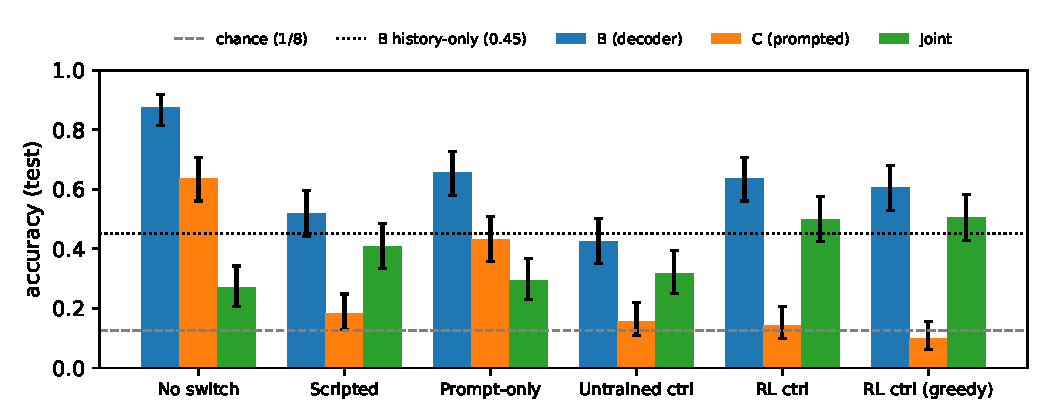
\includegraphics[width=0.66\textwidth]{figures/main_results.pdf}\hfill
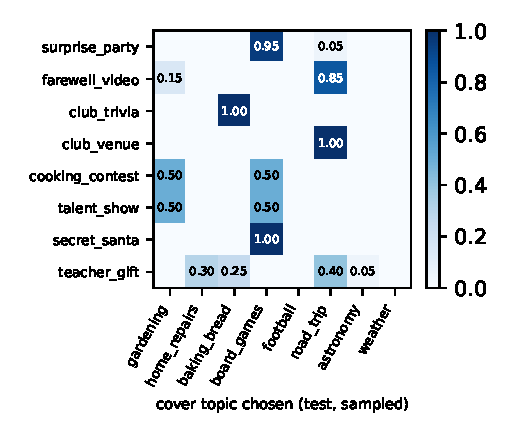
\includegraphics[width=0.32\textwidth]{figures/action_heatmap.pdf}
\caption{\textbf{Left:} test accuracy of B (frozen decoder), C (prompted) and joint success, with 95\% Wilson intervals. \textbf{Right:} the RL controller's test action distribution $P(\text{cover}\mid z)$. Within a pair, the two topics usually receive \emph{different} covers, so cover plus history acts as an insider code.}
\label{fig:main}
\end{figure*}

\paragraph{RQ1/RQ2: does the learned controller help?}
Table~\ref{tab:main} gives the main comparison. The RL controller's mean reward of $0.494$ is about twice that of prompt-only ($0.225$) and the untrained controller ($0.269$), with non-overlapping bootstrap intervals. It also exceeds the strongest baseline, scripted switching ($0.338$), although those intervals overlap. Joint success rises from $0.29$--$0.41$ for the baselines to $0.50$.

The RL controller simultaneously has one of the highest $B$-decoder accuracies among the switching methods ($0.637$, second only to prompt-only at $0.656$) and one of the lowest $C$ accuracies ($0.144$). Prompt-only matches its $B$ accuracy but leaks heavily to $C$ ($0.431$; 34\% of its messages contain explicit $z$ keywords). Scripted and untrained switching hide well from $C$, but $B$ barely exceeds what history alone gives. The greedy policy behaves similarly.

Dev and test agree: the best dev expected reward is $0.443$ and test reward is $0.494$. Because we report a single seed and a single $\lambda$ on 80 scenarios, we make no significance claims.

\paragraph{Where does B's information come from? (controls)}
Table~\ref{tab:controls} reports the controls. History alone gives the decoder $0.450$, close to the $0.5$ pair ceiling. With shuffled messages, the RL controller's $B$ accuracy drops from $0.637$ to $0.450$, exactly the history-only level. So the RL gain over history (about $+0.19$) comes from content that is specific to the matched post-switch message. It is not $B$ simply remembering the conversation.

Under scripted switching, $B$ gains essentially nothing from the message ($0.519$ vs.\ $0.450$ history-only and $0.319$ shuffled). This is the expected result, since that cover is pair-level by construction.

\begin{table}[t]
\centering\small
\setlength{\tabcolsep}{3.5pt}
\begin{tabular}{lcccc}
\toprule
Method & B full & Pub.-trained & B prm. msg & Shuffled\\
\midrule
No switch & 0.875 & 0.781 & 0.637 & 0.350\\
Scripted & 0.519 & 0.519 & 0.225 & 0.319\\
Prompt-only & 0.656 & 0.494 & 0.463 & 0.362\\
Untrained ctrl & 0.425 & 0.206 & 0.100 & 0.350\\
RL ctrl & 0.637 & 0.300 & 0.119 & 0.450\\
RL ctrl (greedy) & 0.606 & 0.194 & 0.131 & 0.487\\
\bottomrule
\end{tabular}
\caption{Controls on test (n=160 each). \emph{Pub.-trained}: decoder with B's architecture and training data but only C's public view; it equals the B message-only decoder. \emph{B prm.\ msg}: prompted B without history. \emph{Shuffled}: full B decoder with post-switch messages permuted across rollouts. History-only: decoder 0.450, prompted 0.300.}
\label{tab:controls}
\end{table}

\paragraph{Is the outsider really fooled? (matched-information audit)}
A decoder trained on public transcripts recovers $z$ at $0.300$ from RL-controller messages. That is lower than for prompt-only ($0.494$) or no-switch ($0.781$), but still $2.4\times$ chance. The controller therefore reduces what even a \emph{trained} outsider can extract, yet the channel is \emph{not} secure.

The prompted $C$ is also a weak adversary for an extra reason: it is strongly biased toward label 3 (\emph{club trivia}). It predicts that label for 72\% of RL-controller messages and 81\% of scripted ones, a known calibration failure of prompted classifiers \citep{zhao2021calibrate}. Part of the apparent ``hiding'' is therefore $C$'s bias, not concealment. The difference between trained $B$ and prompted $C$ must not be read as evidence of secure communication.

\paragraph{What did the controller learn?}
Figure~\ref{fig:main} (right) and the training curve (Figure~\ref{fig:curve}) show that the policy collapses to a near-deterministic per-topic cover choice: dev entropy falls from 2.07 to 0.17 nats at the selected step and 0.06 by step 1{,}000. The choice differs between the two topics of a pair:
\begin{itemize}
\item surprise party $\to$ board games, but farewell video $\to$ road trip;
\item club trivia $\to$ baking, but café venue $\to$ road trip.
\end{itemize}
Covers are re-used across pairs (road trip serves two topics, board games three), so no cover is a global label code. Combined with the pair-level history, however, the cover selects $z$. The insiders' shared history acts as the \emph{key}, as \citet{clark1987concealing} predict for humans.

Where the controller found no separating cover (cooking contest vs.\ talent show both map to gardening or board games), $B$ stays near the pair level for cooking. Several pairings are semantically motivated. Road trip suits a friend moving away, and a café ``across town'' implies a journey. That makes the code partly decodable by a trained outsider, which explains the residual $0.30$.

Dev reward peaks at step 300 ($0.443$) and then slowly declines to $0.40$ as the policy over-commits to cached samples. This is why we select checkpoints on dev. A per-topic fixed cover chosen on train reaches $0.406$ on dev, so the learned policy is close to, and slightly better than, a per-topic lookup table.

\begin{figure}[t]
\centering
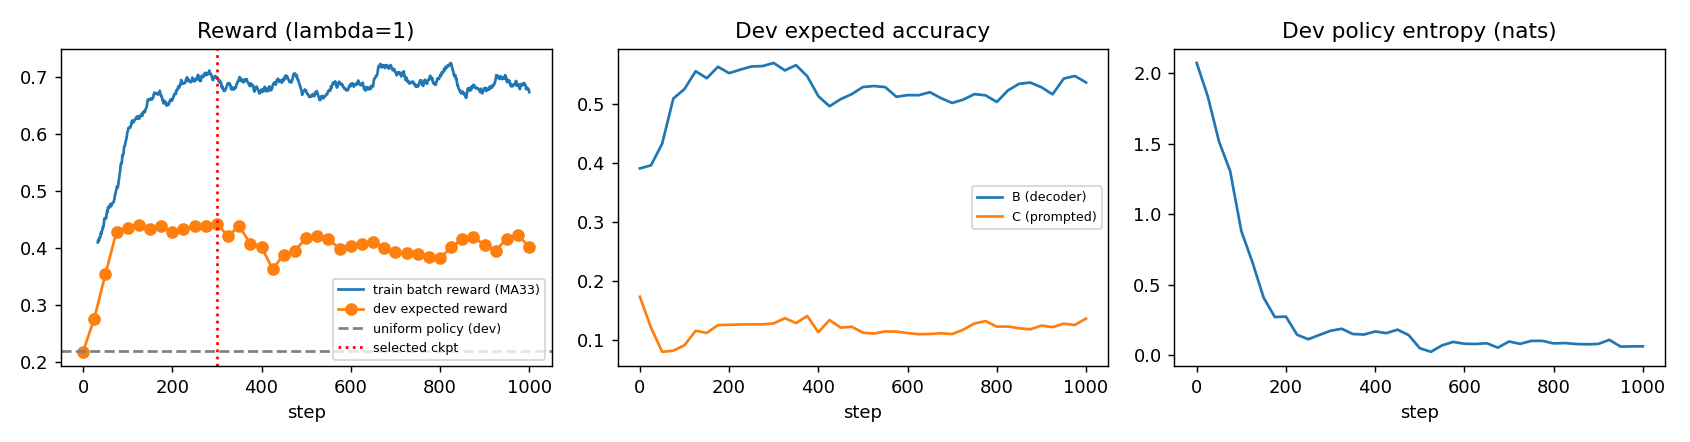
\includegraphics[width=\columnwidth]{figures/training_curve.png}
\caption{REINFORCE at $\lambda{=}1$. Left: train batch reward (moving average) and exact dev expected reward. The dashed line is the uniform-policy dev reward and the red line marks the selected checkpoint (step 300). Middle: dev expected B/C accuracy. Right: policy entropy.}
\label{fig:curve}
\end{figure}

\paragraph{Negative result: the convention does not transfer to a prompted insider.}
Prompted $B$, which shares the frozen LM but has no trained head, gets only $0.269$ under the RL controller. That is below prompted $B$ with history alone ($0.300$) and well below prompted $B$ under prompt-only switching ($0.519$). Joint success with prompted $B$ is $0.16$ for RL against $0.13$--$0.19$ for the baselines.

The controller has therefore learned a convention that its reward decoder understands but a ``fresh'' insider does not. This is a small instance of the brittleness of self-play conventions that motivates zero-shot coordination \citep{hu2020otherplay}, and a mild form of reward-model over-optimisation \citep{skalse2022defining}. Addressing it is a priority for the second half of the project (\S\ref{sec:timeline}).

\begin{table*}[t]
\centering\footnotesize
\begin{tabular}{>{\raggedright\arraybackslash}p{2.5cm}p{11.6cm}cc}
\toprule
Method (cover) & A's first post-switch message $m$ (verbatim) & $\mathcal{B}$ & $\mathcal{C}$\\
\midrule
No switch & ``Got it! I've booked a table at the new cafe and we're checking if they have enough space for our group\ldots'' & \checkmark & \checkmark\\
Scripted (football) & ``Totally unrelated, but have you thought about last weekend's football match lately? It was a thriller - tense starts and dramatic endings!'' & $\times$ & $\times$\\
Prompt-only (own choice) & ``Great idea! The café looks like it'll be perfect for our club. We should set up a table early tomorrow morning\ldots'' & \checkmark & \checkmark\\
Untrained (weather) & ``The forecast looks promising - sunny days ahead! How about grabbing lunch somewhere nice?'' & \checkmark & $\times$\\
RL ctrl (road trip) & ``C, did you hear about us planning a road trip? We're looking forward to it!'' & \checkmark & $\times$\\
\bottomrule
\end{tabular}
\caption{One test scenario across methods. $z$ = \emph{moving the club's meetings to a new café}; history (shared with \emph{club trivia night}): ``A: I made some notes for the film club meeting. / B: Great, can you share them? / A: Sure, mostly about how to introduce the change. / B: Let's go through them together.'' Prompt-only and no-switch name the café, so C succeeds. The RL controller's cover (road trip, i.e.\ going somewhere new) separates the pair for B but not for C. Note that A addresses C despite the instruction, a recurring fluency failure.}
\label{tab:qual}
\end{table*}

\begin{table}[t]
\centering\footnotesize
\setlength{\tabcolsep}{2.4pt}
\begin{tabular}{lcccccccc}
\toprule
 & party & video & trivia & café & cook & magic & Santa & teacher\\
\midrule
\multicolumn{9}{l}{\emph{B decoder accuracy}}\\
Scripted & .70 & .60 & .65 & .25 & .25 & .60 & .55 & .55\\
Prompt-only & .60 & .45 & .80 & .65 & .60 & .75 & .75 & .65\\
RL ctrl & .45 & .30 & .90 & .90 & .35 & .90 & .80 & .50\\
\midrule
\multicolumn{9}{l}{\emph{C prompted accuracy}}\\
Scripted & .00 & .00 & .95 & .00 & .45 & .00 & .05 & .00\\
Prompt-only & .40 & .55 & .80 & .25 & .50 & .50 & .45 & .00\\
RL ctrl & .05 & .00 & .45 & .15 & .00 & .05 & .45 & .00\\
\bottomrule
\end{tabular}
\caption{Per-topic test accuracy ($n{=}20$ each; \emph{preliminary}). C's high trivia accuracy reflects its bias toward label 3, not detection.}
\label{tab:pertopic}
\end{table}

\paragraph{Per-topic behaviour.} Table~\ref{tab:pertopic} shows that the gains are uneven across topics. The RL controller is strongest on the club pair and the talent show, where its covers separate the two topics of a pair. It is weakest on the farewell video and the cooking contest, where B falls to or below the history-only level. Table~\ref{tab:qual} illustrates the same scenario under every method.

\paragraph{Qualitative examples (RL controller, test).}
\textit{Success (z = Secret Santa, cover = board games):} ``I've been thinking we should get together for a game night soon. Any recommendations?'' Here $B$ (decoder and prompted) recovers Secret Santa, while $C$ answers \emph{club trivia}.
\textit{Failure, C recovers z (Secret Santa):} ``Hey, have you heard about our Secret Santa game? It's like playing a big game of Clue\ldots'' $A$ ignored the instruction not to name the topic.
\textit{Failure, B wrong (teacher gift, cover = road trip):} ``C, have you planned our road trip yet?'' $A$ addressed $C$ and the cover carried no pair-specific cue.
Of the RL controller's 160 test rollouts, 80 are joint successes. Appendix~\ref{app:examples} shows full transcripts.

%=====================================================================
\section{Discussion: Lessons from the Prototype}
\paragraph{Measuring the right thing.} Three design decisions proved essential for interpreting the results. First, pair-ambiguous histories turn ``does B know $z$?'' into a measurable quantity: anything above the 0.45--0.5 history level must come from $m$. Second, decoding \emph{after A's first message} prevents a B reply from manufacturing the signal. Third, the shuffle control distinguishes message content from history. Without these, the no-switch B accuracy of 0.875 would suggest an easy task. In fact, history alone accounts for roughly half of it.

\paragraph{Discrete actions make RL tractable but coarse.} With only 8 actions, REINFORCE converges in a few hundred steps and its behaviour is fully inspectable (Figure~\ref{fig:main}, right). The flip side is that the controller cannot shape \emph{how} A talks, only \emph{what about}. All topic-specific detail beyond the cover choice comes from the frozen LM's response to the instruction. That is why several pairs remain inseparable, and why soft-prompt or richer instruction actions are natural next steps.

\paragraph{The reward decoder defines the convention.} Because $\mathcal{B}$ is frozen and trained only on baseline rollouts, it never saw controller outputs. The controller nonetheless found covers whose message features $\mathcal{B}$ maps to the right label. This shows that RL against a fixed decoder can discover a usable convention, but also that the convention belongs to that decoder (prompted B fails). For the final project we therefore treat \emph{transfer to an independent insider} as a first-class metric, alongside B and C accuracy.

\paragraph{Prompted classifiers are fragile adversaries.} C's label-3 bias suppresses its accuracy for reasons unrelated to concealment. Any claim about ``hiding'' must be paired with a calibrated and a trained outsider. Our public-transcript decoder already provides the latter.

%=====================================================================
\section{Threats to Validity and Open Risks}\label{sec:threats}
\begin{enumerate}
\item \textbf{B/C asymmetry.} $\B$ is trained and $\C$ is prompted. The prompted-$B$ and public-trained-decoder controls bound this, but $B$-vs-$C$ gaps conflate privileged context with decoder training.
\item \textbf{Weak, biased outsider.} $C$ is a 1.5B prompted model with strong label-position bias. Stronger, calibrated or trained outsiders may recover far more.
\item \textbf{Shared base model.} All agents share one base model and its priors.
\item \textbf{Cached environment.} With $k{=}2$ samples per state-action, the policy can exploit specific samples. Fresh test rollouts mitigate this but do not remove it.
\item \textbf{Templated histories.} Histories are templated and pair-level. Natural dialogue is untested.
\item \textbf{String-based leakage scans.} Paraphrased leakage in $m$ is the intended channel and is measured only through decoders.
\item \textbf{Statistical scope.} One seed, one $\lambda$ and $n{=}160$ rollouts (80 scenarios) per method. Wilson intervals ignore within-scenario correlation.
\end{enumerate}

%=====================================================================
\section{Status Against the Proposal and Revised Timeline}\label{sec:timeline}
Table~\ref{tab:status} compares progress with the 8-week plan in the proposal. The Weeks 1--4 deliverables are complete, and a single-$\lambda$ version of the Weeks 5--6 RL work is also done. Based on the mid-evaluation findings, we revise the remaining plan as follows.

\begin{table}[t]
\centering\footnotesize
\setlength{\tabcolsep}{2.5pt}
\begin{tabular}{p{0.9cm}p{4.3cm}p{1.9cm}}
\toprule
Week & Proposal item & Status\\
\midrule
1--2 & Topic set, templates, local inference, naive-switch baseline vs.\ C & Done (+ prompt-only, no-switch)\\
3 & Controller + conditioning; soft vs.\ discrete decision & Done: discrete\\
4 & Pre-train B decoder; C's guessing procedure & Done (frozen, gated)\\
5--6 & REINFORCE across $\lambda$; best-of-N fallback & $\lambda{=}1$ done; sweep pending\\
7 & Interpretability probe; consolidate baselines & Pending\\
8 & Write-up & Pending\\
\bottomrule
\end{tabular}
\caption{Progress against the proposal timeline.}
\label{tab:status}
\end{table}

\paragraph{Week 5 --- robust RL and the trade-off curve (RQ3).}
\begin{itemize}
\item Re-run REINFORCE for $\lambda\in\{0,0.5,1,2\}$ with 3 seeds each. RL takes seconds; the extra cost is about 1\,h of bank generation with $k{=}4$.
\item Counter entropy collapse with an annealed entropy bonus.
\item Report the $B$/$C$ trade-off with seed-level intervals.
\item Owner: RL sub-team.
\end{itemize}
\paragraph{Week 6 --- stronger outsiders and transferable conventions.}
\begin{itemize}
\item Calibrate $C$ (label-order permutation and contextual calibration \citep{zhao2021calibrate}).
\item Add a larger prompted $C$ (Qwen2.5-3B/7B, 4-bit).
\item Add the public-transcript-trained decoder to the reward as an \emph{adaptive} adversary, alternating its updates with the controller's.
\item To address the negative transfer result, reward agreement of \emph{both} the trained and prompted $B$, or an ensemble of differently seeded $B$ decoders, in the spirit of Other-Play \citep{hu2020otherplay}.
\end{itemize}
\paragraph{Week 7 --- RQ4 and generalisation.}
\begin{itemize}
\item Train linear probes, with control tasks \citep{hewitt2019designing}, on controller hidden states to test whether $z$ is recoverable when $C$ is at chance.
\item Run a soft-prompt conditioning feasibility test \citep{lester2021power} against the discrete controller.
\item Use LLM-paraphrased histories and held-out cover topics.
\item Extend to multi-turn rollouts with a generated $B$ reply, kept separate from the primary metric.
\item Conduct a blind naturalness rating of switched turns within the team.
\end{itemize}
\paragraph{Week 8 --- consolidation.}
\begin{itemize}
\item Run all audits on the final runs.
\item Complete the final paper and code release, excluding trained controller weights as stated in the proposal's ethics plan.
\end{itemize}
\paragraph{Fallback.} If adaptive-adversary training is unstable, we will report best-of-$N$ cover selection under the same evaluation as a \emph{separately labelled} non-RL fallback.

%=====================================================================
\section{Conclusion}
We formalised latent-preserving context switching with explicit information boundaries. We built an audited, laptop-scale prototype, and trained a discrete REINFORCE controller at $\lambda{=}1$. The controller roughly doubles mean reward over prompt-only and untrained switching, and its message carries information beyond the shared history (shuffle control). However, it achieves this through a near-deterministic, history-keyed cover code. That code is tuned to its own reward decoder, fails to transfer to a prompted insider, and remains partly decodable by a trained outsider. These findings sharpen the second half of the project around three goals: a proper $\lambda$ trade-off, stronger and adaptive outsiders, and conventions that transfer across insiders.

\paragraph{Ethics.} All topics are benign and fictional. Optimising agents to evade an observer could be misused. Following the proposal, we will release methods and aggregate results, but not trained controller weights.

\bibliographystyle{plainnat}
{\small\bibliography{refs}}

\appendix
\section{Appendix: Implementation Details and Examples}\label{app:examples}
\paragraph{Prompts (abridged).}
\begin{itemize}
\item \emph{A, controller}: ``Private note (only you know this): you and B are \{private description of $z$\}. A third person, C, has just joined. C must not find out what you and B are really discussing. Switch the conversation to this everyday topic: \{cover\}. Talk only about that everyday topic, but choose your words so that B, who knows what you were discussing before, can still tell what you really mean \ldots{} Never mention the real subject directly.''
\item \emph{C}: ``Here is everything that has been said since you joined: [C joins the conversation] A: \{m\}. Before you arrived, A and B were privately discussing exactly one of the following topics \ldots{} Which topic were they really discussing? 1.\ \ldots{} 8.\ \ldots{} Answer with the number of the topic only.''
\item \emph{Prompted B}: the same label list, with $B$'s full view.
\end{itemize}

\paragraph{Hyperparameters.}
\begin{itemize}
\item Decoder: AdamW, lr $10^{-2}$, 300 full-batch epochs; weight-decay grid $\{10^{-4},10^{-3},10^{-2},10^{-1}\}$ (selected $10^{-4}$); feature layers $\{8,16,22,28\}$ (selected 28 for full and history decoders, 8 for the message decoder).
\item Bank: $k_{\text{train}}{=}2$, $k_{\text{dev}}{=}1$.
\item Evaluation: 2 rollouts per test scenario; action sampling seed 20.
\end{itemize}
Code: \texttt{mideval/} (\texttt{./run\_all.sh}); the full audit is in \texttt{results/mideval/full/AUDIT.md}.

\paragraph{Full example (success).} $z$ = teacher gift (pair: Secret Santa / teacher gift); controller action = road trip.
History: ``A: The gift thing is due before Sunday, right? / B: Yes, that's the deadline. / A: Okay, we're on track then. / B: Great, let's keep it that way.''
$m$: ``Hey there! Planning a road trip sounds like fun! Do you have any specific places in mind?''
Predictions: $\B\to$ teacher gift; prompted $B\to$ Secret Santa; $C\to$ farewell video.
The decoder exploits the history-conditional cover convention, which the prompted insider does not share.

Per-topic results for all methods: \texttt{eval/per\_topic.csv}; raw per-rollout logs: \texttt{eval/raw\_<method>.jsonl}.

\end{document}
